% !TEX root = ../foresight.tex

\section{Relative pose localization}

\begin{figure}
  \centering
    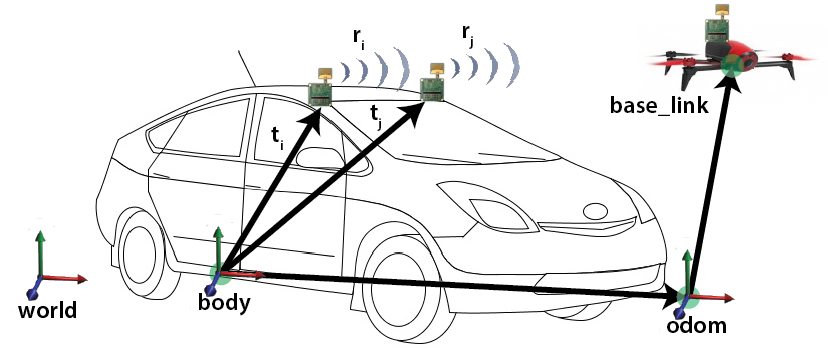
\includegraphics[width=0.45\textwidth]{foresight_frames}
  \caption{The frames and measurements of our system. The base frame
   is the car's body frame. We measure transforms $t_{i}$ from the body
   frame to every UWB tag. The velocity controller uses the odom-to-base\textunderscore 
   link transform to calculate commands to control the quadcopter's velocity.
   Planning is done in the car's body frame.
   The UWBs make range measurements $r_{i}$. A position estimate $\hat{x}$
   is calculated by solving for the least squares error between $r_{i}$ and $\hat{x}$.}
  \label{fig:frames}
\end{figure}

We use 6 ultra-wideband radios and the Bebop's onboard odometry measurements
to estimate the relative position of the quadcopter with respect to the car with an
accuracy of +/- 6cm. The 6 UWBs were positioned as far apart as possible on the
car while still generally maintaining line of sight with the quadcopter when the
quadcopter is positioned in front of the car. The transform from a set base position
on the car to each UWB was then measured. These transforms allow us to
calculate the distance between each UWB and the estimated state of the quadcopter.

Orientation is calibrated at start by lining up the quadcopter along the car's x-axis.
We rely on the Bebop's onboard yaw measurement for orientation.
We collect the range measurements $r_{i}$ from the 6 UWBs (at a rate of about 10 Hz)
and use nonlinear least squares optimization to estimate the quadcopter's x-y position. 
We combine the x-y position estimate with altitude and velocity data from the quadcopter in
a UKF provided by the ROS robot\textunderscore localization package.  We found that
the UWB range data was not reliable enough to accurately calculate the z position
from the range data alone. We therefore use the z value estimated by the UKF in
the nonlinear least squares optimization.